\documentclass{beamer}
\usepackage[utf8]{inputenc}

\usetheme{Madrid}
\usecolortheme{default}
\usepackage{amsmath,amssymb,amsfonts,amsthm}
\usepackage{txfonts}
\usepackage{tkz-euclide}
\usepackage{listings}
\usepackage{adjustbox}
\usepackage{array}
\usepackage{tabularx}
\usepackage{gvv}
\usepackage{lmodern}
\usepackage{circuitikz}
\usepackage{tikz}
\usepackage{graphicx}

\setbeamertemplate{page number in head/foot}[totalframenumber]

\usepackage{tcolorbox}
\tcbuselibrary{minted,breakable,xparse,skins}



\definecolor{bg}{gray}{0.95}
\DeclareTCBListing{mintedbox}{O{}m!O{}}{%
  breakable=true,
  listing engine=minted,
  listing only,
  minted language=#2,
  minted style=default,
  minted options={%
    linenos,
    gobble=0,
    breaklines=true,
    breakafter=,,
    fontsize=\small,
    numbersep=8pt,
    #1},
  boxsep=0pt,
  left skip=0pt,
  right skip=0pt,
  left=25pt,
  right=0pt,
  top=3pt,
  bottom=3pt,
  arc=5pt,
  leftrule=0pt,
  rightrule=0pt,
  bottomrule=2pt,

  colback=bg,
  colframe=orange!70,
  enhanced,
  overlay={%
    \begin{tcbclipinterior}
    \fill[orange!20!white] (frame.south west) rectangle ([xshift=20pt]frame.north west);
    \end{tcbclipinterior}},
  #3,
}
\lstset{
    language=C,
    basicstyle=\ttfamily\small,
    keywordstyle=\color{blue},
    stringstyle=\color{orange},
    commentstyle=\color{green!60!black},
    numbers=left,
    numberstyle=\tiny\color{gray},
    breaklines=true,
    showstringspaces=false,
}
%------------------------------------------------------------
%This block of code defines the information to appear in the
%Title page
\title %optional
{4.5.14}
\date{September  2025}
%\subtitle{A short story}

\author % (optional)
{BEERAM MADHURI - EE25BTECH11012}



\begin{document}


\frame{\titlepage}
\begin{frame}{Question}
Solve the system of equations\\
\begin{align*}
    2x + y &=5\\
    3x+2y &=8
\end{align*}
\end{frame}
 
\begin{frame}{solution}
    \frametitle{finding the solution of given equations : }
The equation of line:
\begin{align}
n^\top x = c
\end{align}
Line L:
\begin{align}
\begin{pmatrix}2 & 1\end{pmatrix}\begin{pmatrix}x \\y\end{pmatrix}= 5
\end{align}

Line K:
\begin{align}
\begin{pmatrix}3 & 2\end{pmatrix}\begin{pmatrix}x \\y\end{pmatrix}= 8
\end{align}
Writing in matrix form:
\begin{align}
\begin{pmatrix}2 & 1 \\3 & 2\end{pmatrix}\begin{pmatrix}x \\y\end{pmatrix}=\begin{pmatrix}5 \\8\end{pmatrix}
\end{align}
\end{frame}
\begin{frame}
The following augmented matrix can be solved by gaussian elimination
\begin{align}
\begin{pmatrix}2 & 1 & | & 5 \\3 & 2 & | & 8\end{pmatrix}\xrightarrow{R_2 \to R_2 - \frac{3}{2}R_1}\begin{pmatrix}2 & 1 & | & 5 \\0 & \frac{1}{2} & | & \frac{1}{2}\end{pmatrix}
\end{align}
Since,
\begin{align}
\rank(A) = \rank(A|b) = 2
\end{align}
the system has a unique solution.

from $2^{\text{nd}}$ row,
\begin{align}
y = 1 \Rightarrow x = 2
\end{align}

$\therefore$ Solution of given system of equations is:$\begin{pmatrix}x \\y\end{pmatrix}$= $\begin{pmatrix}2 \\1\end{pmatrix}$
\end{frame}

\begin{frame}[fragile]
\frametitle{Python Code}
\begin{lstlisting}
import numpy as np
import matplotlib.pyplot as plt

# Create a range of x-values for plotting
x = np.linspace(-2, 6, 400)

# Rearrange the equations to solve for y
# Equation 1: 2x + y = 5  =>  y = 5 - 2x
y1 = 5 - 2 * x
\end{lstlisting}
\end{frame}

\begin{frame}[fragile]
\frametitle{Python Code}
\begin{lstlisting}
# Equation 2: 3x + 2y = 8  =>  2y = 8 - 3x  =>  y = (8 - 3x) / 2
y2 = (8 - 3 * x) / 2
# --- Create the Plot ---
plt.figure(figsize=(10, 8))
# Plot the two lines
plt.plot(x, y1, label=r'$2x + y = 5$')
plt.plot(x, y2, label=r'$3x + 2y = 8$')
\end{lstlisting}
\end{frame}

\begin{frame}[fragile]
\frametitle{Python Code}
\begin{lstlisting}
# The solution is the intersection point (2, 1)
solution_x = 2
solution_y = 1

# Plot and annotate the intersection point
plt.plot(solution_x, solution_y, 'ro', markersize=8, label=f'Solution ({solution_x}, {solution_y})')
plt.annotate(f'({solution_x}, {solution_y})', 
             xy=(solution_x, solution_y), 
             xytext=(solution_x + 0.2, solution_y + 0.2))
\end{lstlisting}
\end{frame}

\begin{frame}[fragile]
\frametitle{Python Code}
\begin{lstlisting}
# --- Formatting the Graph ---
plt.title('Solution of the System of Equations', fontsize=16)
plt.xlabel('x-axis', fontsize=12)
plt.ylabel('y-axis', fontsize=12)
plt.axhline(0, color='black', linewidth=0.5)
plt.axvline(0, color='black', linewidth=0.5)
plt.grid(True, which='both', linestyle='--', linewidth=0.5)
plt.legend(fontsize=12)
plt.show()
\end{lstlisting}
\end{frame}

\begin{frame}[fragile]
\frametitle{C Code}
\begin{lstlisting}
#include <stdio.h>

int main() {
// The given system of equations is:
// 2x + 1y = 5
// 3x + 2y = 8

// Define the coefficients and constants from the equations
// Equation 1: a1*x + b1*y = c1
\end{lstlisting}
\end{frame}

\begin{frame}[fragile]
\frametitle{C Code}
\begin{lstlisting}
double a1 = 2.0, b1 = 1.0, c1 = 5.0;
// Equation 2: a2*x + b2*y = c2
double a2 = 3.0, b2 = 2.0, c2 = 8.0;

// Variables to store the solution
double x, y;
// Calculate the determinant of the coefficient matrix
// D = (a1 * b2) - (a2 * b1)
double determinant = a1 * b2 - a2 * b1;
\end{lstlisting}
\end{frame}

\begin{frame}[fragile]
\frametitle{C Code}
\begin{lstlisting}
if (determinant != 0) {
x = (c1 * b2 - c2 * b1) / determinant;
y = (a1 * c2 - a2 * c1) / determinant;
printf("The solution is:\n");
printf("x = %.2f\n", x);
printf("y = %.2f\n", y);
    } else {
printf("The system does not have a unique solution.\n");
    }
    return 0;
}
\end{lstlisting}
\end{frame}

\begin{frame}[fragile]
\frametitle{Python and C Code}
\begin{lstlisting}
from ctypes import c_double

def solve_linear_system():
    # Coefficients and constants from the equations
    a1 = c_double(2.0)
    b1 = c_double(1.0)
    c1 = c_double(5.0)

    a2 = c_double(3.0)
    b2 = c_double(2.0)
    c2 = c_double(8.0)
\end{lstlisting}
\end{frame}

\begin{frame}[fragile]
\frametitle{Python and C Code}
\begin{lstlisting}
    # Calculate the determinant
    determinant = c_double(a1.value * b2.value - a2.value * b1.value)

    if determinant.value != 0:
        # Use Cramer's Rule
        x = c_double((c1.value * b2.value - c2.value * b1.value) / determinant.value)
        y = c_double((a1.value * c2.value - a2.value * c1.value) / determinant.value)
\end{lstlisting}
\end{frame}

\begin{frame}[fragile]
\frametitle{Python and C Code}
\begin{lstlisting}
        # Print the results
        print("The solution is:")
        print(f"x = {x.value:.2f}")
        print(f"y = {y.value:.2f}")
    else:
        print("The system does not have a unique solution.")
# Run the function
solve_linear_system()

\end{lstlisting}
\end{frame}
\begin{frame}
\begin{figure}
    \centering
    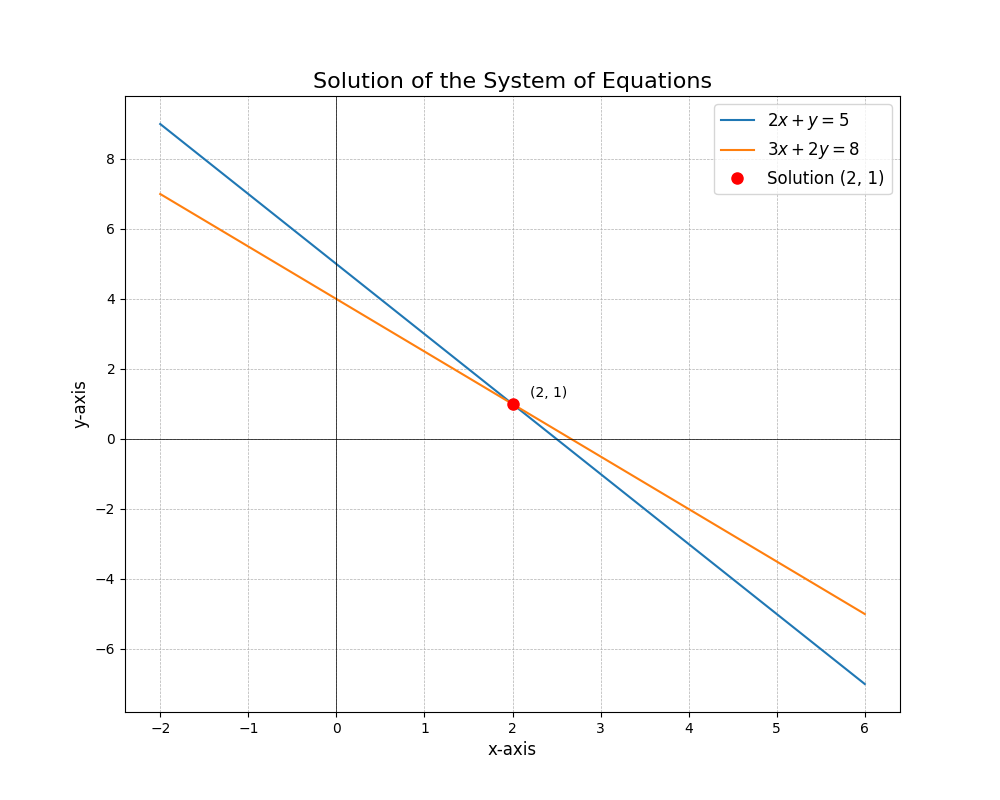
\includegraphics[width=0.75\columnwidth]{graph10.png}
    \caption{Plot}
    \label{fig:Line}
\end{figure}
\end{frame}

\end{document}